\documentclass[letterpaper,12pt]{article}
\usepackage[utf8]{inputenc}
\usepackage[spanish]{babel}
\usepackage{fontenc}
\usepackage{graphicx}
\usepackage{anysize}
\usepackage{amsmath}
\marginsize{3cm}{2cm}{1cm}{1cm}
\usepackage[dvips]{hyperref}
\title{OPEN ERP Modulo OCS (Office of Citizen Service)\\Manual de Usuario}
\author{Andrés Ignacio Báez, Cinxgler Mariaca\\Revisado por: \\
Angel María Fonseca Correa (SubDirector de Recursos Tecnológicos - IDU)}
\date{Noviembre de 2012}
\begin{document}
\maketitle
%%Introduccion sobre que es El software Libre y que es OpenErp, y la licencia AGPL OCS de forma General
%\section{Introducción}
\subsection{¿Qué es software libre?}
El software libre es aquel que respeta la libertad de los usuarios y de la comunidad, si se afirma de un programa de computadora que es software libre, es porque 
garantiza que se cumplan las cuatro libertades fundamentales que menciona la Free Software Foundation\cite{GNU}:
\begin{itemize}
 \item La libertad de ejecutar el programa para cualquier propósito.
 \item La libertad de estudiar cómo funciona el programa, y cambiarlo para que haga lo que usted quiera. 
 \item La libertad de redistribuir copias para ayudar a su prójimo.
 \item La libertad de distribuir copias de sus versiones modificadas a terceros. Esto le permite ofrecer a toda la comunidad la oportunidad de 
 beneficiarse de las modificaciones. El acceso al código fuente es una condición necesaria para ello. 
\end{itemize}
Por estas razones cuando se dice que un programa esta hecho en Java, $C\#$ o Python, no significa que sea software libre, si como usuario o cliente del software no
se garantiza el respeto integral de estas cuatro libertades. 
\subsection{¿Qué es un Erp?}
Un ERP (Planificacion de Recursos Empresariales) es el principal activo de software que tiene una empresa, ya que es un sistema de información que se encarga
de registrar las actividades de negocio, su enfoque debe estar orientado a la misionalidad de la organización. En un ERP básicamente se lleva  
la contabilidad, los presupuestos, la producción, ventas, recursos humanos, proyectos, etc. Ejemplos de ERP a usados a nivel local son SIIGO, DMS, STONE, SAP, Softland, etc.\\
Muchos errores directivos en las organizaciones es que no adquieren su software ERP para registrar y controlar sus actividades misionales, sino que se limitan al área 
administrativa (contabilidad,presupuestos, etc), generando desconexión entre los procesos y propiciando riesgos de desorden que hacen perder eficiencia a la organización.\\
La implementación de un software ERP dentro de una empresa es en general un proceso demorado y costoso, y su éxito se convierte en un factor crítico para que 
una compañía logre cumplir sus objetivos de negocio. 
\subsection{¿Que es OpenErp?}
OpenErp es un ERP de talla mundial, distribuido bajo la filosofia del software libre con la licencia AGPL.
La orientación de su desarrollo es módular, es decir que 
se instalan solamente las cosas que se necesitan concretamente para la organización, se puede comenzar instalando una aplicación y luego 
agregar otros módulos más adelante.\\
De esta manera los usuarios obtienen los beneficios de un software integrado. Los modulos desarrollados incluyen Ventas,
CRM (Customer Resource Management), gestión de proyectos, gestión de almacenes, fabricación, gestión financiera, recursos humanos sólo por nombrar algunos. 
Más de 700 módulos de OpenERP están disponibles en internet \cite{OpenErp}.

\subsection{¿Qué significa la licencia AGPL?}
La licencia  Pública General de GNU (GPL) es la vía legal que permite a los usuarios garantizar las cuatro libertades fundamentales del software libre.
La licencia pública general de Affero (en inglés, Affero General Public License, también Affero GPL o AGPL) es una licencia 
derivada de la Licencia (GPL) la cúal fue diseñada específicamente para asegurar la cooperación con la comunidad
en el caso de software que corra en servidores de red.\\
La Affero GPL es íntegramente una GNU GPL con una cláusula nueva que añade la obligación de distribuir el software si éste se 
ejecuta para ofrecer servicios a través de una red de ordenadores\cite{AGPLexp}.

\subsection {¿Qué es el Módulo OCS?}
El módulo Office Of Citizen Services, (Oficina de Atencion al Ciudadano) es un módulo orientado para organizaciones públicas que están obligadas a 
atender peticiones de la ciudadanía, el módulo sirve para registrar las PQR que 
ingresan por los diferentes canales.\\
Para consolidar el análisis de las PQR, se incluye un componente de georrefenciación, que permite que la información 
sea consultada desde un Sistema de Información Geográfica como Quantum o gvSIG.\\
No se incluye el componente de gestión documental. 
%%Introducción sobre el módulo desde la perspectiva del IDU
%%\section{Presentación del Sistema de Gestión de PQRs}

El Sistema de Gestión de PQRs para el IDU es una extensión del módulo Office Of Citizen Services (Oficina de Atencion al Ciudadano) disponible 
en la plataforma de Software Libre OpenERP, 
el objetivo de este sistema es el de brindar a las organizaciones públicas que están obligadas a 
atender solicitudes de la ciudadanía una herramienta que permita registrar las PQR que ingresan por los diferentes canales y manejar su ciclo de vida
dentro de la organización, desde la creación hasta la finalización de la PQR donde se da la respuesta al ciudadano.\\
Adicionalmente, se incluye un componente de georeferenciación, que permite que la información 
sea consultada desde un Sistema de Información Geográfica como Quantum o gvSIG, esta característica permite realizar análisis geográficos de las PQRs registradas.\\

\subsection{Funcionalidad e integración con otros sistemas}

\begin{figure}[h]
 \centering6
 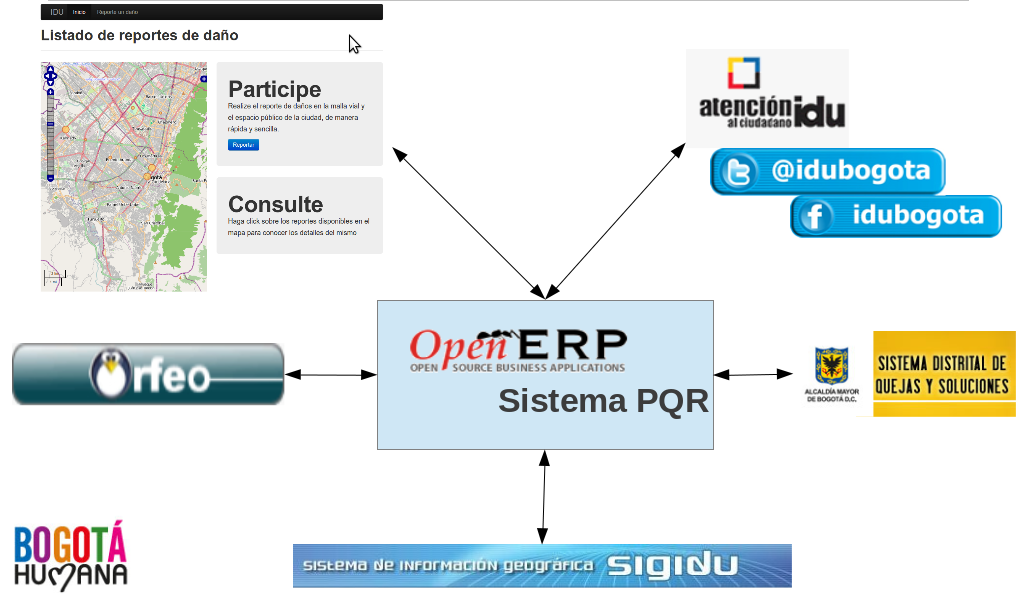
\includegraphics[width=17cm,height=9.5cm]{./Imagenes/slidesistemacompleto.png}
 % Login.png: 1289x610 pixel, 96dpi, 34.10x16.14 cm, bb=0 0 967 457
 \caption{Perspectiva actual del sistema OpenERP dentro del IDU}
 \label{fig:slidesistemacompleto}
\end{figure}

Al interior del IDU el sistema de PQRs se integra a los demás sistemas de información tal como se ve en la figura \ref{fig:slidesistemacompleto}. OpenERP consolida la 
información de todas las PQR que ingresan al instituto por los diversos canales. A su vez cuenta con los mecanismos para comunicarse con los otros sistemas de información 
relacionados: Sistema de Información Geográfico del IDU (SIGIDU), Sistema de Gestión Documental (Orfeo GPL), Sistema Distrital de 
Quejas y Soluciones (SDQS).\\

Las PQRs se tramitan de la siguiente manera: Se registran en OpenERP, allí son gestionadas por la Oficina de atención al ciudadano,
si no se cuenta con una respuesta inmediata, pasan a la dependencia relacionada de la organización a través del
sistema de Gestión Documental Orfeo, OpenERP espera la respuesta y conserva el número de radicación de Orfeo. Los casos y los documentos, son copiados también 
a SDQS, lo cual es necesario para cumplir la normativa Distrital.\\

El ciudadano dispone de una herramienta para registrar su PQR desde el portal Web Institucional, se trata del portal de Huecos,
desde ahí se diligencia un formulario con toda la información relacionada a los daños de la malla vial, se hace una clasificación y se ubica el 
punto en el mapa de la ciudad. El reporte es almacenado en OpenERP y luego tramitado.(Esta funcionalidad se encuentra en desarrollo)\\

Si un ciudadano llega personalmente a las instalaciones del IDU y radica un documento, este es digitalizado, ingresa al sistema Orfeo, si el 
documento se cataloga como una PQR, pasa automáticamente a OpenERP para que sea tramitado.(Esta funcionalidad se encuentra en desarrollo)\\

Si el ciudadano ingresa a la página de Internet de SDQS y crea una petición, esta es remitida al IDU por servicios Web, ingresa directamente a OpenERP, 
y allí se inicia el trámite correspondiente.(Esta funcionalidad se encuentra en desarrollo)\\


%%Contenido del módulo base de acuerdo a los estados...
%
%		Este Modulo Explica como se registra la PQR
%
\section{Uso del Módulo OCS (Usuario)}

\subsection{Ingreso al Sistema}
%%%%%%%%%% Imagen del Login
\begin{figure}[h]
 \centering
 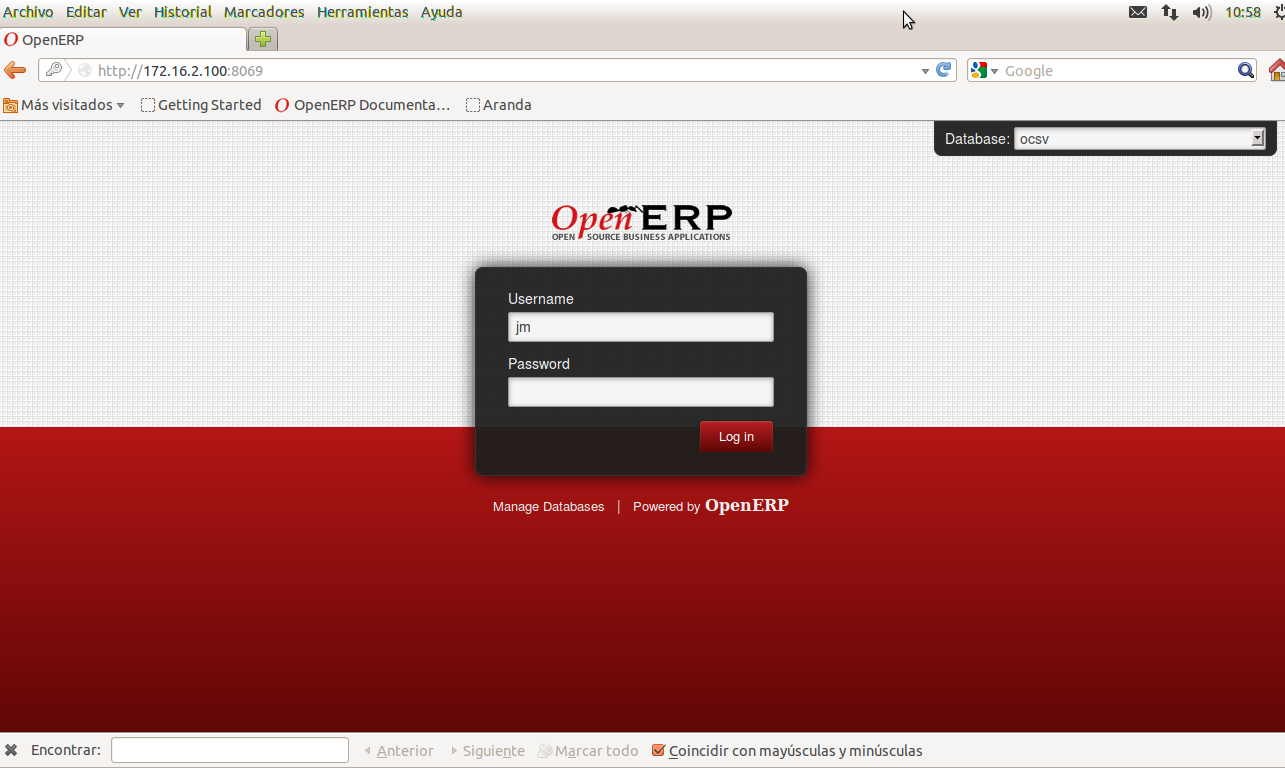
\includegraphics[width=17cm,height=10cm]{./Imagenes/Login.png}
 % Login.png: 1289x610 pixel, 96dpi, 34.10x16.14 cm, bb=0 0 967 457
 \caption{Pantalla de Inicio}
 \label{fig:login}
\end{figure}

%%%%%%%%% Imagen de los modulos de la aplicación

\begin{figure}[h]
 \centering
 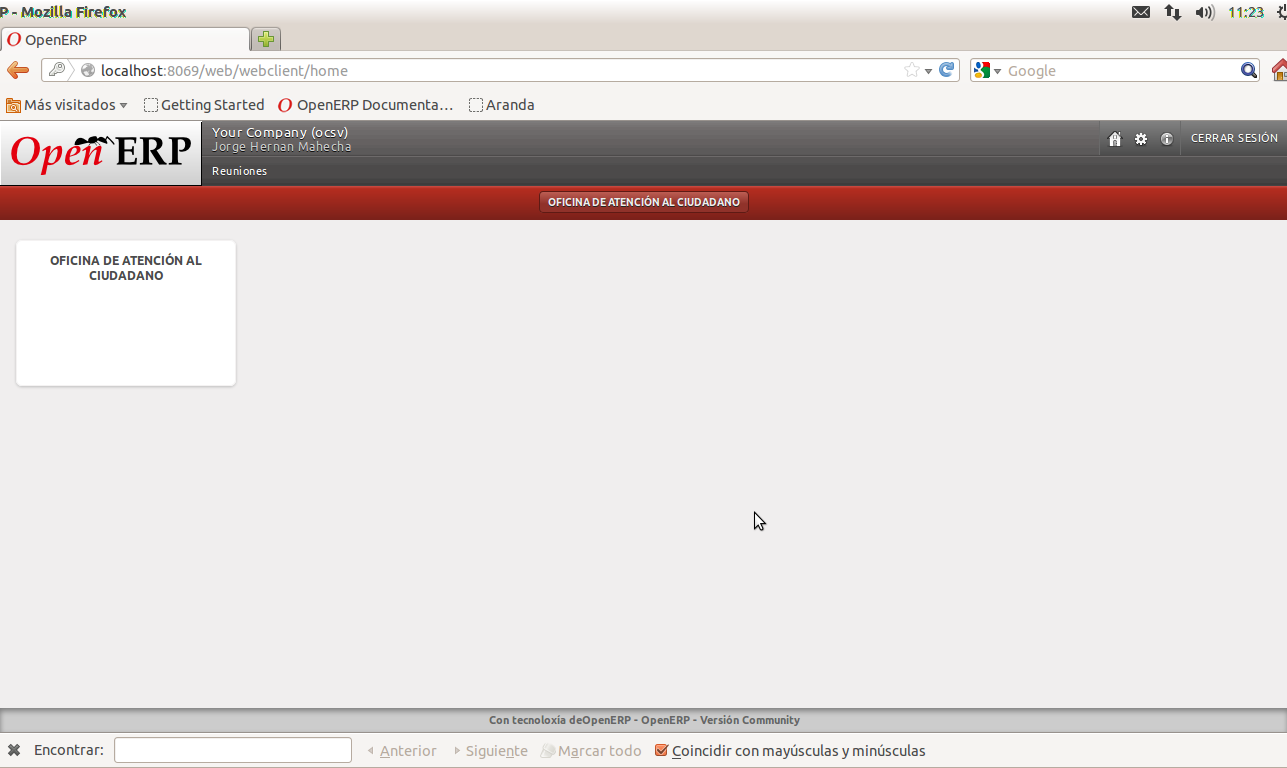
\includegraphics[width=17cm,height=10cm]{./Imagenes/menumain.png}
 % Login.png: 1289x610 pixel, 96dpi, 34.10x16.14 cm, bb=0 0 967 457
 \caption{Menú Principal de la aplicación}
 \label{fig:menumain}
\end{figure}

\begin{itemize}
 \item Para ingresar al sistema utilice un navegador (ej: mozilla firefox, chrome), y en la barra de direcciones coloque la ruta del servidor: \underline{http://172.16.2.180:8069}. Aparecerá la pantalla
 de inicio que se ve en la figura \ref{fig:login}
 \item Ingrese los datos de su cuenta, login y password.
 \item Si los datos de la cuenta son correctos, la siguiente pantalla muestra el menú principal de la aplicación (figura \ref{fig:menumain}).
 \item Hacer clic en el menú Oficina de Atención al ciudadano $\Rightarrow$ PQR.
 \item Aparecerá la lista con las PQR que deben ser tramitadas por el usuario (figura \ref{fig:menulista}).
\end{itemize}


\subsection {Tramite de una PQR}

\begin{figure}[h]
 \centering
 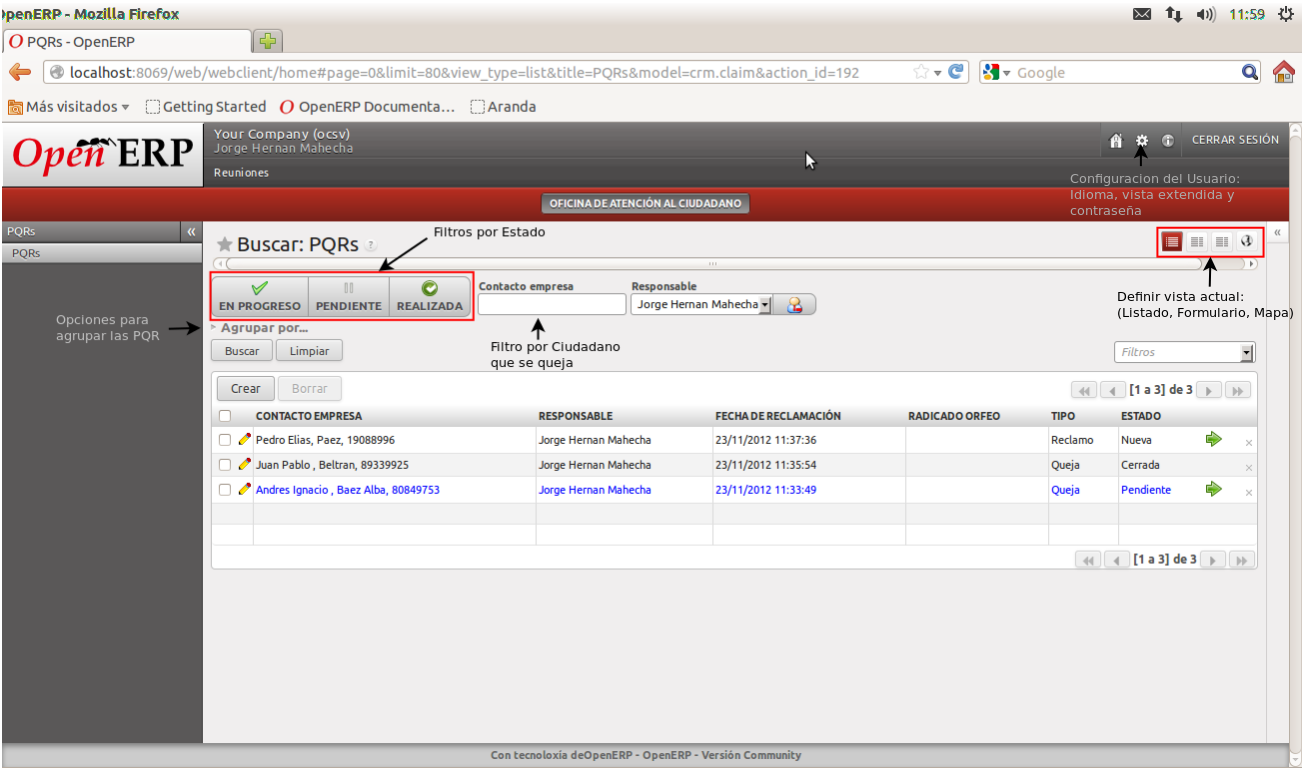
\includegraphics[width=17cm,height=10cm]{./Imagenes/menulista.png}
 % Login.png: 1289x610 pixel, 96dpi, 34.10x16.14 cm, bb=0 0 967 457
 \caption{Listado de PQR}
 \label{fig:menulista}
\end{figure}


\begin{figure}
 \centering
 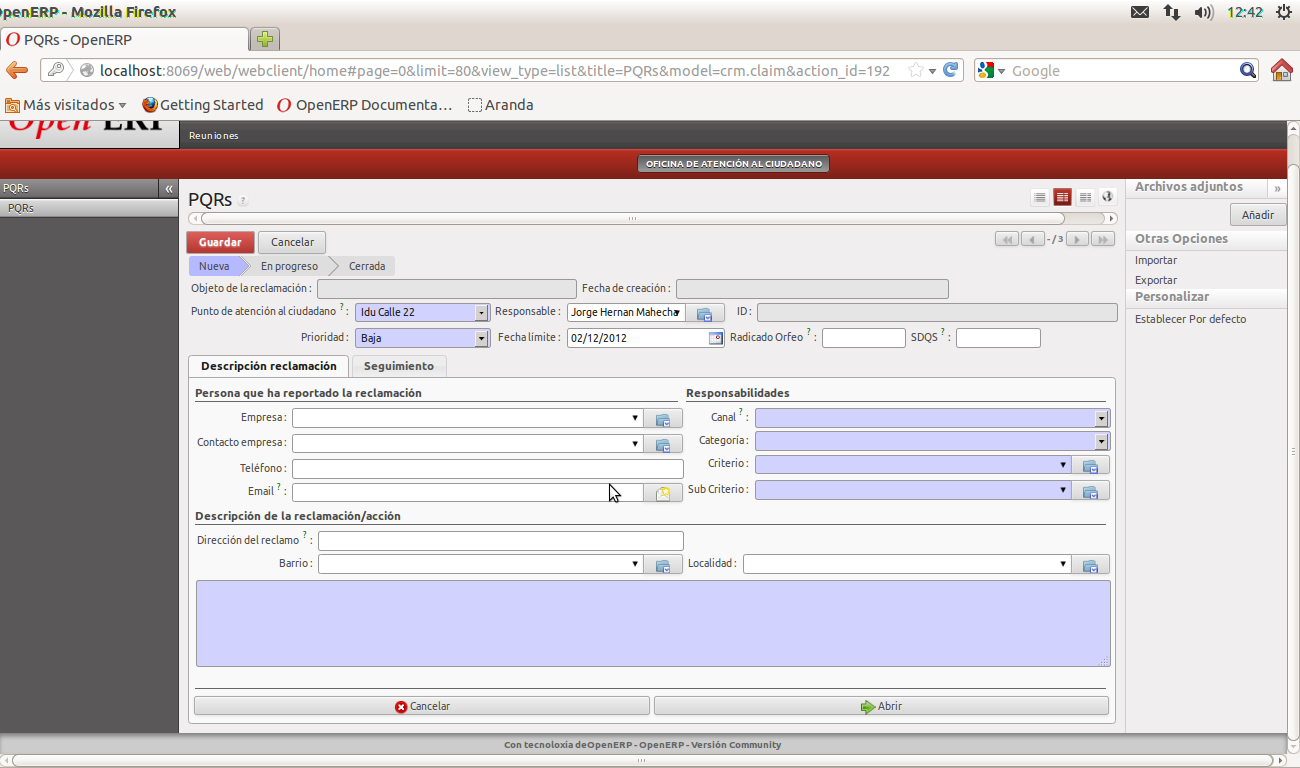
\includegraphics[width=17cm,height=10cm]{./Imagenes/formularioregistro.png}
 % Login.png: 1289x610 pixel, 96dpi, 34.10x16.14 cm, bb=0 0 967 457
 \caption{Registro inicial de la PQR}
 \label{fig:formularioregistro}
\end{figure}

\subsubsection{Estados de las PQR}

Antes de registrar las PQR, es importante tener en cuenta que éstas se clasifican por estados, 
el estado ayuda a conocer como va el trámite en el que se encuentra la PQR, de esta manera controlar su gestión.\\

Si se trata de un borrador, la PQR se graba como \textbf{nuevo}, si la PQR ya se encuentra en trámite y la respuesta que se puede dar es casi inmediata
su estado será en \textbf{progreso}, si la PQR no se puede responder rápidamente, debe pasar a un estado \textbf{pendiente}, y si ya se le ha contestado al ciudadano, 
el estado es \textbf{cerrado}, una vez se cierra la PQR ésta no se puede modificar, y su reapertura está reservada para la persona que coordina el 
grupo de usuarios.

\subsubsection{Creación de una PQR}

Para realizar el registro de una PQR se deben seguir los siguientes pasos:

\begin{itemize}
 \item Hacer clic en Oficina de Atención al Ciudadano $\Rightarrow$ PQR. 
 \item Hacer clic en el botón \textbf{Crear} que aparece en la grilla de la Lista, ver figura \ref{fig:menulista} 
 \item Aparecerá el formulario de la figura \ref{fig:formularioregistro}. Los datos que se deben ingresar son: El usuario que registra 
 la pqr (por defecto), el punto de atención donde se lleva a cabo dicha digitación (IDU, Cade), una prioridad, la fecha límite para tener la respuesta, el número
 de radicación en Orfeo si se tiene y el número de radicado de SDQS (Sistema Distrital de Quejas y Soluciones) si se tiene \footnote{En la actualidad 
 se está desarrollando el módulo para llevar a cabo dicho proceso automáticamente}. 
 \item En el campo para anotar los datos de la persona que hace la reclamación, se pueden presentar varios casos: 
 \begin{enumerate}
  \item La queja es anónima: en tal caso los campos donde se relacionan empresa y contacto van vacíos. 
  \item La queja es interpuesta por una empresa: se deben llenar los datos de ésta, y relacionar una persona de contacto. Para ello se deben llenar 
  los datos de la empresa, haciendo clic en el icono a la derecha del campo 
  \textbf{Empresa} , luego clic en \textbf{Crear}. Aparece una ventana emergente en donde se registran los
  datos básicos de la empresa (ver figura \ref{fig:pantempresa}), como lo es el nombre y el NIT (que se almacenará en el campo $CIF\backslash NIF$) 
  y \textbf{Guardar}. Se regresa a la pantalla anterior (figura \ref{fig:formularioregistro}. 
  En el campo contacto, se hace clic en el icono de la derecha y luego \textbf{Crear}. Aparecerá el formulario de la figura \ref{fig:formusuario}.
  En este formulario se ingresan los datos de la persona: Tipo de Documento, Numero de Documento, Primer Nombre, Segundo Nombre, la 
  empresa (Es la misma empresa que se acaba de ingresar), el cargo que desempeña en la empresa, y algún dato de contacto. Para que la 
  persona se pueda registrar, debe entregar al menos un dato de contacto.  Luego se hace clic en guardar.    
  \item La queja es interpuesta por una persona natural: Se ingresan los datos de la persona, para ello se hace clic en el icono a la izquierda  
  del campo contacto $\Rightarrow$ \textbf{Crear} y luego diligenciar el formulario de la figura \ref{fig:formusuario}.
 \end{enumerate}
 \item En el area señalada como responsabilidades, se selecciona el \textbf{Canal} por donde llegó la PQR, el \textbf{tipo de requerimiento},
 el \textbf{criterio} y \textbf{subcriterio} (\textbf{Tipificación}). Los subcriterios varían de acuerdo al criterio seleccionado, por tando es importante seleccionar
 primero el criterio, si no ve el criterio dentro las primeras opciones, puede ir escribiendo el texto hasta que aparezca en el cuadro el valor deseado, o 
 si no, simplemente hacer clic en el botón a la derecha y luego en \textbf{Buscar}. Allí se desplega un cuadro donde se puede seleccionar
 el criterio o subcriterio de una manera más cómoda (Ver figura \ref{fig:buscarcriterios}).
 
 
 \item Luego llenar los datos de contacto y los criterios, 
 se registra el sitio de la reclamación, la localidad y el barrio, junto con
 el texto de la reclamación y se hace clic en \textbf{Abrir}, en ese momento la reclamación pasa a estado \textbf{en progreso}.
\end{itemize}

\begin{figure}
 \centering
 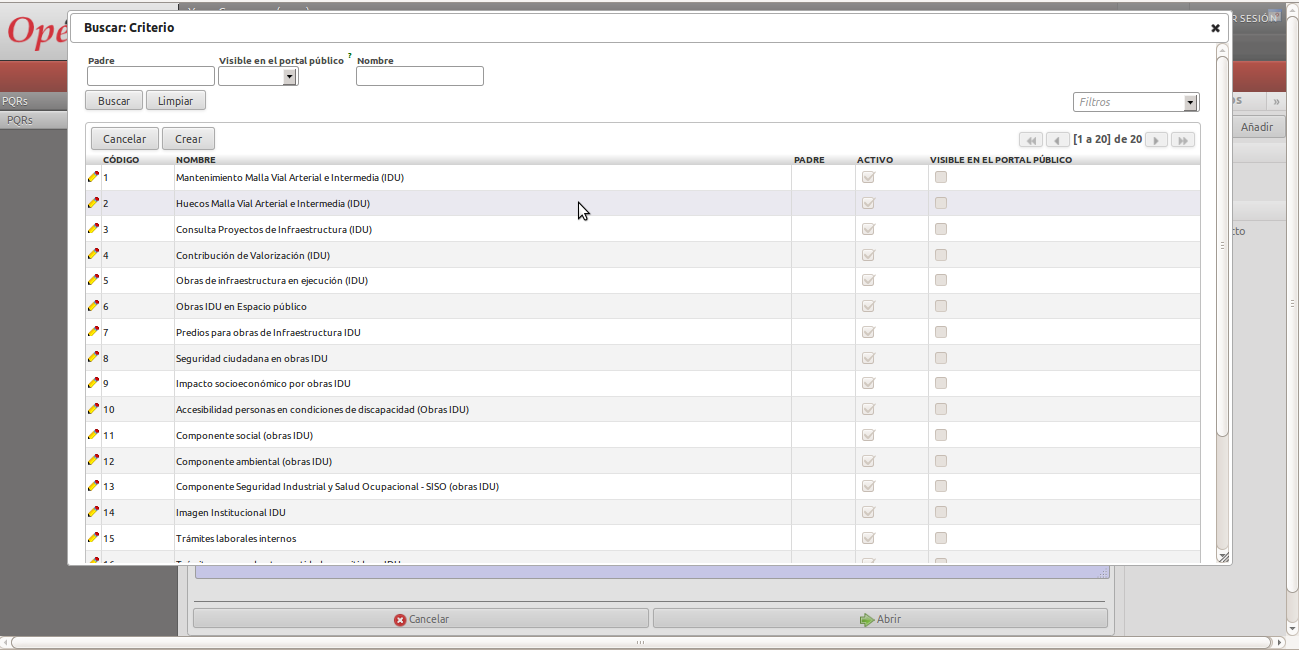
\includegraphics[width=17cm,height=10cm]{./Imagenes/buscarcriterios.png}
 % Login.png: 1289x610 pixel, 96dpi, 34.10x16.14 cm, bb=0 0 967 457
 \caption{Ventana emergente para buscar criterios y subcriterios}
 \label{fig:buscarcriterios}
\end{figure}



\begin{figure}
 \centering
 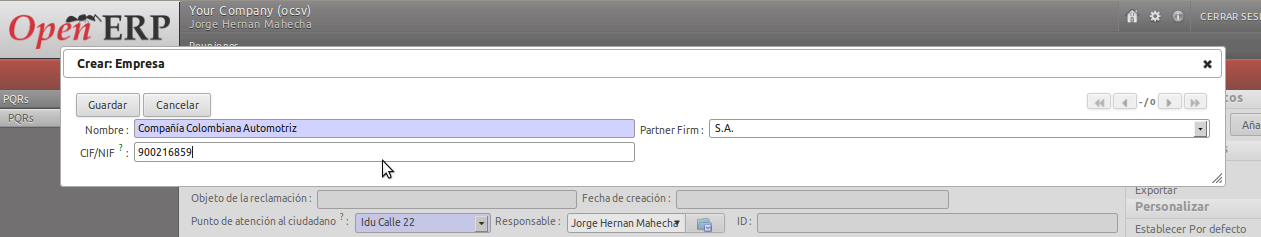
\includegraphics[width=17cm,height=4cm]{./Imagenes/pantempresa.png}
 % Login.png: 1289x610 pixel, 96dpi, 34.10x16.14 cm, bb=0 0 967 457
 \caption{Ventana emergente que solicita datos de la empresa}
 \label{fig:pantempresa}
\end{figure}


\begin{figure}
 \centering
 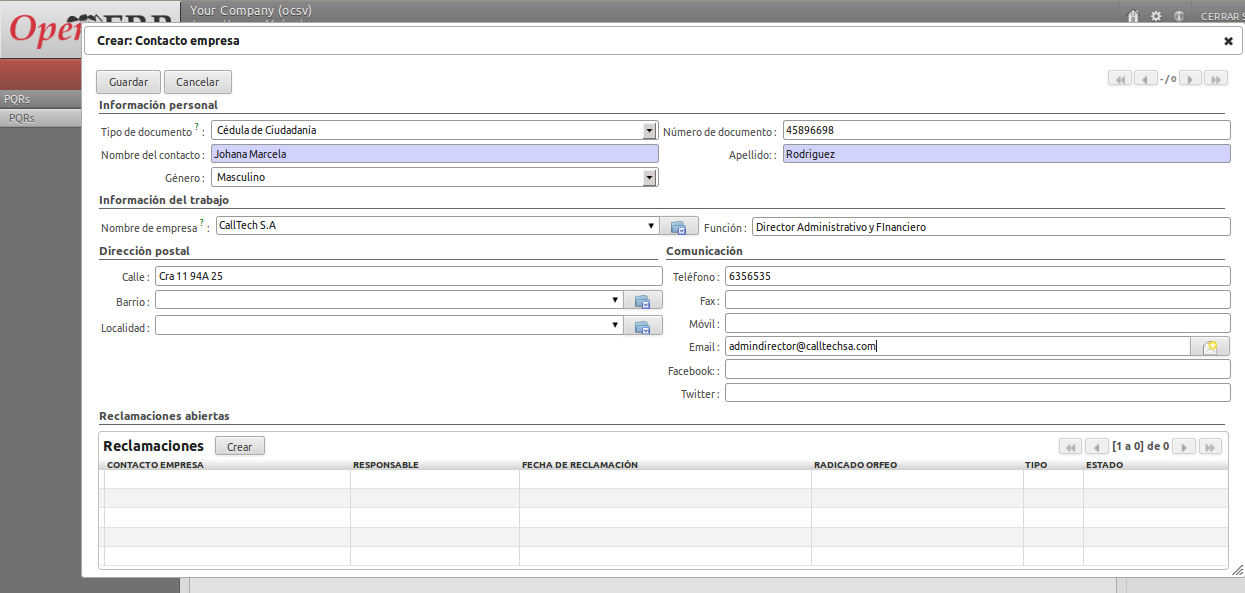
\includegraphics[width=17cm,height=8cm]{./Imagenes/formusuario.png}
 % Login.png: 1289x610 pixel, 96dpi, 34.10x16.14 cm, bb=0 0 967 457
 \caption{Ventana emergente para llenar la información de los ciudadanos}
 \label{fig:formusuario}
\end{figure}

\begin{itemize}
 \item Si no se tiene la respuesta de la PQR a la mano, es importante pasarla a estado pendiente, para ello se hace clic en el botón \textbf{Pendiente} 
que se encuentra en la parte inferior del formulario. 
\item Si la respuesta del caso está se puede obtener en primera instancia, escriba el texto de respuesta en el campo \textbf{Solución} 
que se encuentra en la pestaña \textbf{Seguimiento}. Luego haga clic en el boton \textbf{Realizada} 
que se encuentra en la parte inferior del formulario (figura \ref{fig:formseguimiento}).
\end{itemize}


\subsubsection{Cierre de la reclamación}


\begin{figure}
 \centering
 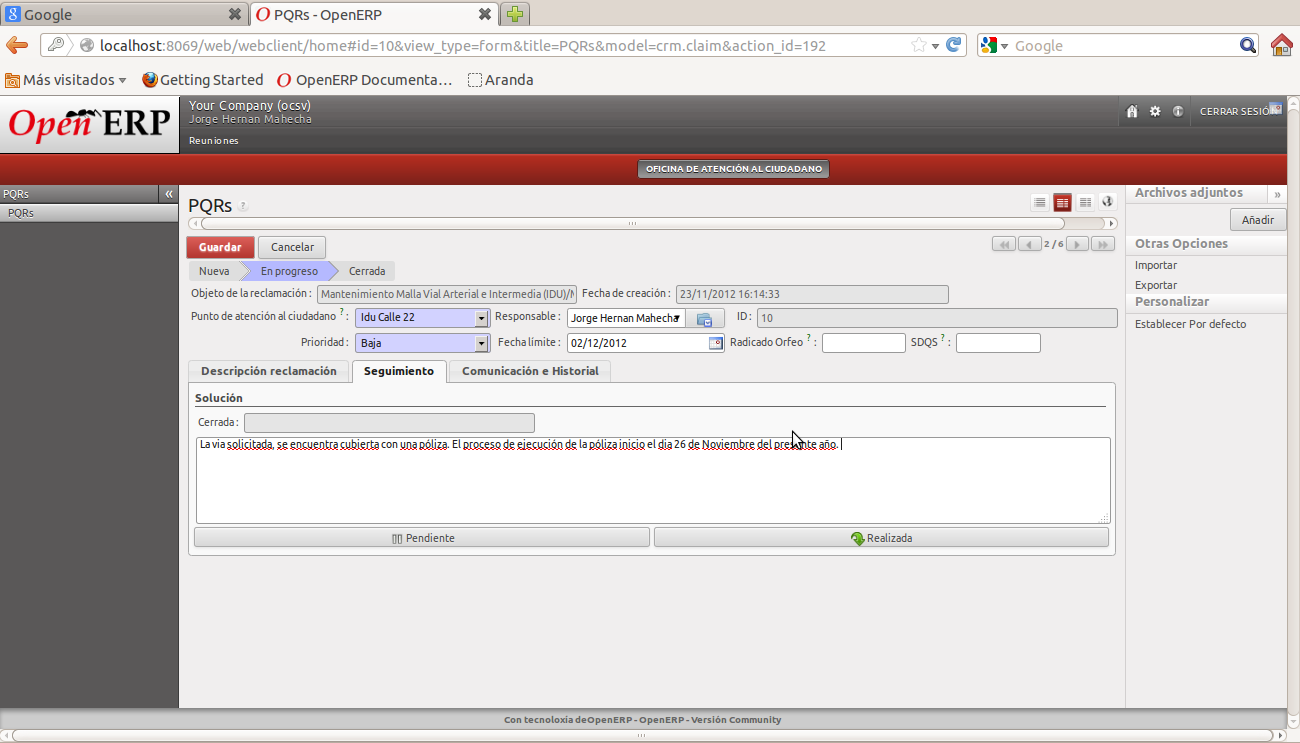
\includegraphics[width=17cm,height=10cm]{./Imagenes/formseguimiento.png}
 % Login.png: 1289x610 pixel, 96dpi, 34.10x16.14 cm, bb=0 0 967 457
 \caption{Formulario de la PQR con el campo para escribir el texto de solución}
 \label{fig:formseguimiento}
\end{figure}

Siga los siguientes pasos para dar respuesta a la PQR:

\begin{itemize}
 \item Hacer clic en \textbf{Oficina de Atención al Ciudadano} $\Rightarrow$ PQR.
 \item En la lista (figura \ref{fig:menulista}) seleccionar el caso respectivo.
 \item Hacer clic en la pestaña \textbf{Seguimiento} y escribir la respuesta en el campo \textbf{Solución}.
 \item Hacer clic en el botón \textbf{Realizada} que se encuentra en la parte inferior del formulario. 
\end{itemize}

\subsection{Agregar Notas a una PQR}


Se pueden agregar anotaciones a la PQR, así com visualizar el historial de las acciones realizadas. Para hacerlo se debe habilitar
la interfaz web en modo extendido: 

\begin{itemize}
 \item Tomando como referencia la figura \ref{fig:menulista} hacer clic en el icono en forma de rueda que se encuentra a la
 izquierda del botón \textbf{CERRAR SESION}.
 \item Aparece un menú emergente de con las preferencias sobre el sistema (figura \ref{fig:configuracion}). En la opcion
  \textbf{Interfaz} seleccionar la opción \textbf{Extendida}. 
 \item Este cambio hace que en general la aplicación muestre más opciones que cuando esta en modo simplificado. Al hacer 
 clic en \textbf{Oficina de Atencion al Ciudadano} $\Rightarrow$ PQR $\Rightarrow$ Clic un caso cualquiera, se puede ver
 que en el formulario de la figura \ref{fig:formularioregistro} aparece la pestaña \textbf{Comunicación e Historial} 
 (figura \ref{fig:historico}). 
 \item Para agregar una nota se debe hacer clic en el botón \textbf{Añadir nota interna}, que aparece sobre la grilla.
 \item Se desplega la ventana ventana emergente de la figura \ref{fig:addnote}. Para añadir la nota se agrega el texto
 texto deseado y luego \textbf{Añadir}. 
\end{itemize}

\begin{figure}
 \centering
 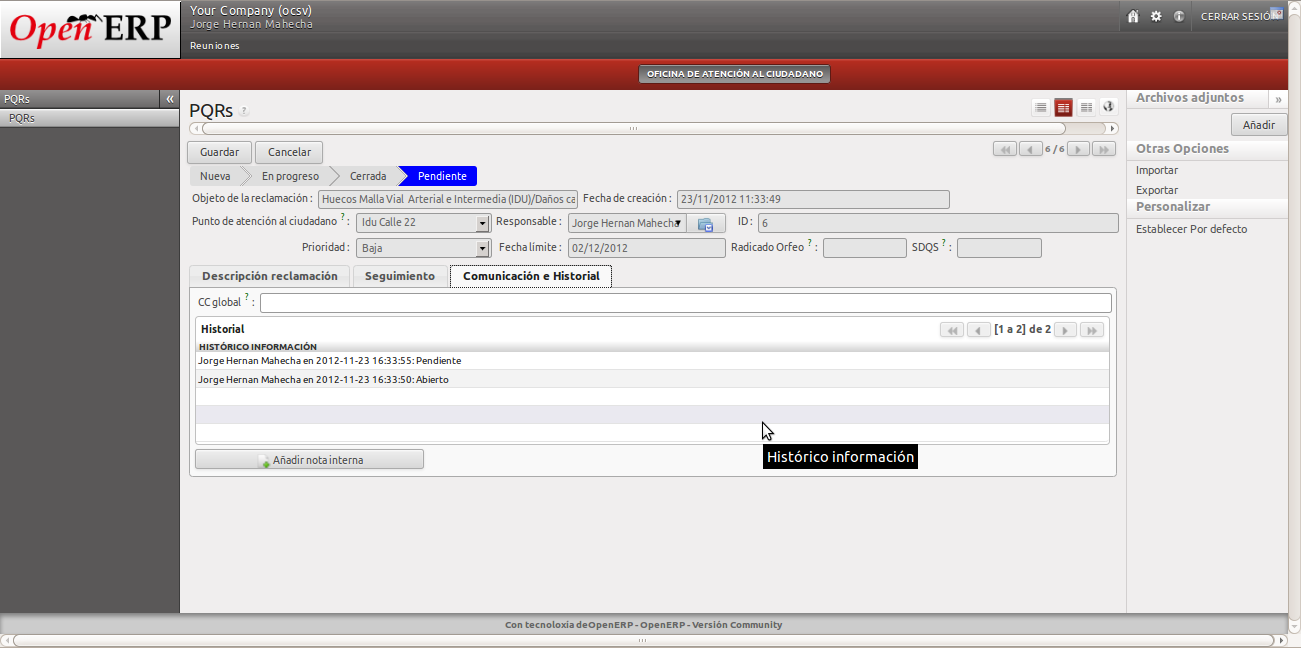
\includegraphics[width=17cm,height=10cm]{./Imagenes/historico.png}
 % Login.png: 1289x610 pixel, 96dpi, 34.10x16.14 cm, bb=0 0 967 457
 \caption{Historico de Acciones en la PQR}
 \label{fig:historico}
\end{figure}


\begin{figure}
 \centering
 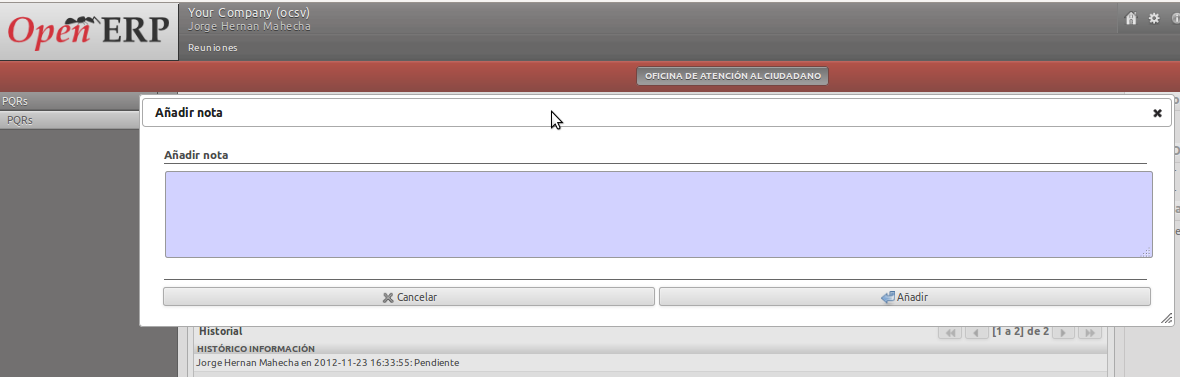
\includegraphics[width=17cm,height=6cm]{./Imagenes/addnote.png}
 % Login.png: 1289x610 pixel, 96dpi, 34.10x16.14 cm, bb=0 0 967 457
 \caption{Ventana Emergente para agregar notas internas}
 \label{fig:addnote}
\end{figure}


\subsection{Uso de la Vista de PQR en modo Lista}

Cuando se está en la vista de PQR en modo lista, se tienen algunas funcionalidades que ayudan a realizar un filtrado rápido de las mismas,
así como funciones de agrupación. 

\begin{figure}
 \centering
 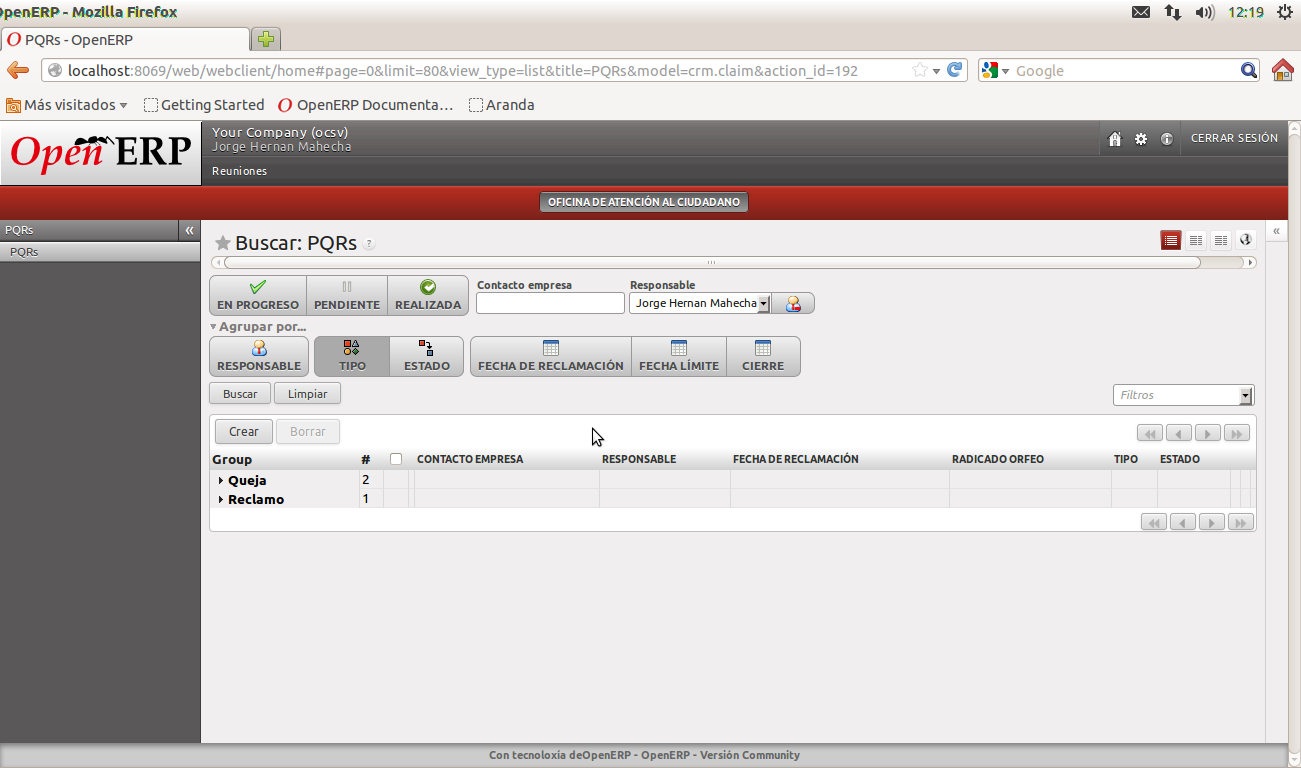
\includegraphics[width=17cm,height=10cm]{./Imagenes/menulistagroup.png}
 % Login.png: 1289x610 pixel, 96dpi, 34.10x16.14 cm, bb=0 0 967 457
 \caption{Agrupando la lista de PQR}
 \label{fig:menulistagroup}
\end{figure}

Para agrupar las PQR hacer clic en el texto \textbf{Agrupar por}, de esta manera puede elegir los siguientes
criterios de agrupación (ver figura \ref{fig:menulistagroup}).
\begin{itemize}
 \item Responsable (Usuario a cargo de la PQR)
 \item Tipo (Petición, Queja, Reclamo, Sugerencia)
 \item Estado (Nuevo, Pendiente, En Progresso, Cerrado)
 \item Fecha de la Reclamación
 \item Fecha Limite
 \item Fecha de Cierre
\end{itemize}









\begin {thebibliography}{1} 
\bibitem{GNU} Free Software Foundation, ¿Qué es software libre?. http://www.gnu.org/philosophy/free-sw.es.html.
\bibitem{OpenErp} Open Erp. De un vistazo. http://www.openerp.com/es/products/at-a-glance
\bibitem{AGPLexp} Explicación de la licencia Affero GPL. \\http://es.wikipedia.org/wiki/GNU\_Affero\_General\_Public\_License 
\bibitem{Agpldef} Definición de la licencia Affero GPL. http://www.gnu.org/licenses/agpl-3.0.html
\end {thebibliography}


\end{document}




